\begin{figure*}[tp]
    \centering
    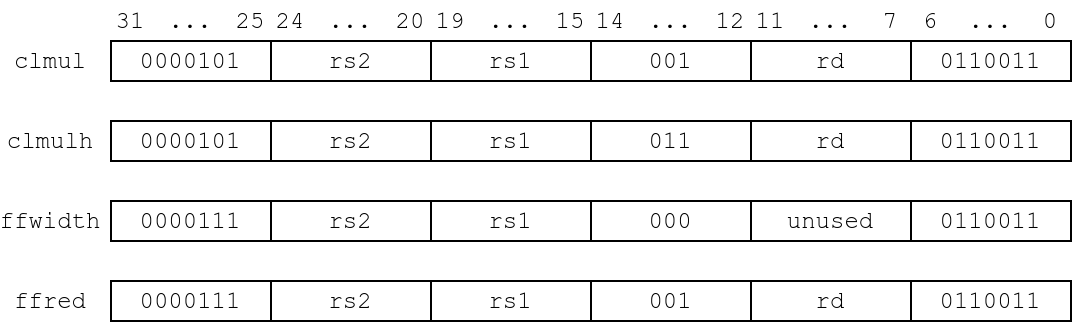
\includegraphics[width=0.8\linewidth]{img/instr.png}
    \caption{The instruction format for the custom galois field arithmetic instructions.}
    \Description{The instruction format for the custom galois field arithmetic instructions.}
    \label{fig:instr}
\end{figure*}

This section describes the ISA extension for RISC-V processors proposed in this work. The selection criteria
of the opcodes were based on the SweRV-EL2 \cite{marena2019risc} microarchitecture. 

The operation added in this extension is the multiplication of finite fields since the sum of two numbers in 
$GF(2^m)$ is only an XOR operation, and it is already defined in RV32I. The multiplication is done in three different 
instructions (See Section \ref{section:gf_mult}): carry-less multiplication (CLMULH and CLMUL) and polynomial reduction (FFRED). 
The carry-less operation requires two instructions since multiplying two 32-bit numbers results in a 64-bit number, 
and the size of the RV32 registers is 32-bit.

To correctly multiply two numbers in $GF(2^m)$, it is also necessary to indicate the irreducible polynomial and the 
degree to the processor. Therefore, additional instruction is required to pass these parameters (FFWIDTH). 
These parameters are stored in two internal registers at the input of the reduction module. The block diagram is shown in Fig. \ref{fig:exu}.

In some processors, such as SweRV-EL2, carry-less multiplication is already implemented in the processor as an extension. Hence, 
the opcode is kept for a compatibility and resource sharing issue.

\begin{figure}[b]
    \centering
    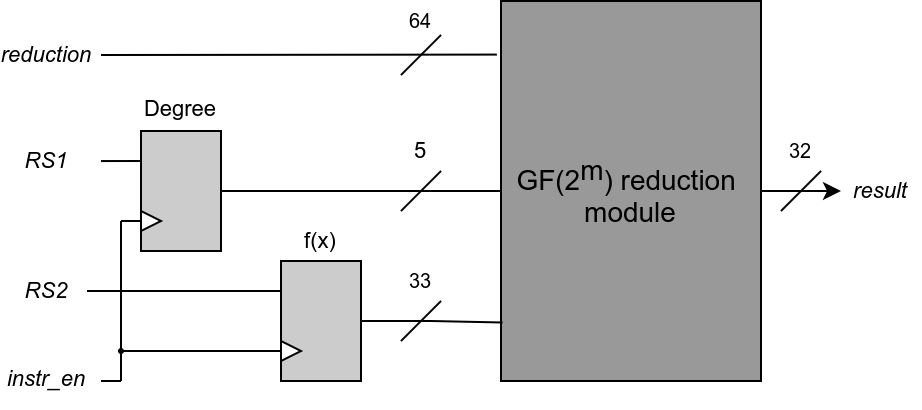
\includegraphics[width=0.95\linewidth]{img/exu.png}
    \caption{FFWIDTH internal registers.}
    \Description{FFWIDTH internal registers.}
    \label{fig:exu}
\end{figure}

We decided not to implement the square function and the inverse of $GF(2^m)$ since they are modules that require much logic 
and can also be calculated using finite field multiplication. In more specific computers, these two instructions can be added to 
improve the system's efficiency at the expense of increasing logic utilization.

Figure \ref{fig:instr} shows the formats of the custom instructions proposed in this work. As we can see here, the carry-less multiplication 
keeps the RISC-V extension B format. 

The parameters that receive and return the instructions are:

\begin{itemize}
    \item \textbf{FFWIDTH}: It receives in RS1 the degree of the polynomials, and in RS2, the irreducible polynomial. 
    These two parameters are stored in internal parameters. Since RV32I registers are 32-bits, 
    the most significant bit of the irreducible polynomial is assumed to be logical 1 when the degree of the input polynomials is 32.
    \item \textbf{FFRED}: It receives the polynomial to be reduced as a parameter. In RS1, it receives the high part, and in RS2, the low part of the polynomial. 
    This instruction returns the reduced polynomial $c(x)$. 
    \item \textbf{CLMULH \& CLMUL}: The parameters are the same as extension B.
\end{itemize}


\begin{lstlisting}[caption={GF multiplication for AES.},captionpos=b,label={lst:aes}]
    li	    a5, 8       % Polynomial degree
    li	    a4,283      % Primitive poly
    ffwidth	a5,a5,a4    
    ...
    lbu	    a4,0(a0)    % Operand A
    lbu	    a7,0(a1)    % Operand B
    clmul	a4,a4,a7    % CL multiplication
    li	    a5,0
    ffred	a7,a5,a4    % Reduction
\end{lstlisting}

\begin{table*}[tp]
    \begin{tabular}{
    >{\columncolor[HTML]{EFEFEF}}c ccc}
    \cellcolor[HTML]{C0C0C0}Instruction          & \cellcolor[HTML]{C0C0C0}Inputs & \cellcolor[HTML]{C0C0C0}Destination register & \cellcolor[HTML]{C0C0C0}Description   \\ \hline
    li a5, 8                                     & 8                              & a5                                           & Load the value 8 in register a5       \\
    li a4, 283                                   & 283                            & a4                                           & Load 283 (primitive poly.) in a4      \\
    ffwidth                                      & a4, a5                         & a5                                           & Store 8 and 283 in internal registers \\
    \vdots & \vdots           & \vdots                         & \vdots                  \\
    lbu                                          & 0(a0)                          & a4                                           & Load operand A in a4                  \\
    lbu                                          & 0(a1)                          & a7                                           & Load operand B in a7                  \\
    clmul                                        & a4, a7                         & a4                                           & CL multiply, result in a4             \\
    li                                           & 0                              & a5                                           & Load 0 in a5                          \\
    ffred                                        & a4, a5                         & a7                                           & Poly. reduction, result in a7        
    \end{tabular}
    \caption{Detailed description of the code in Listing \ref{lst:aes} (AES example).}
    \label{tab:detail}
\end{table*}

An example of the multiplication of finite fields using the custom instructions is shown in Listing \ref{lst:aes}. 
This example is a part of the AES code. AES employs the following reducing polynomial for multiplication:
\begin{equation}
    f(x) = x^{8} + x^{4} + x^{3} + x + 1
    \label{eq:aes}
\end{equation}

This primitive polynomial belongs to $GF(2^8)$. Therefore, the degree is 8. Additionally, this polynomial can represent in binary, 
hexadecimal, or decimal form (see Eq. \ref{eq:aes2}). 
\begin{equation}
    100011011_{2}=11B_{16}=283_{10}
    \label{eq:aes2}
\end{equation}


The number 283 is the value loaded in the second instruction of Listing \ref{lst:aes}, representing the primitive polynomial in base 10.

The FFWIDTH instruction appears only for the first time to tell the hardware 
the degree and the irreducible polynomial. These two received parameters are stored in internal registers. 
Additionally, this instruction receives a value in the result in a5 since the format of FFWIDTH corresponds to an 
operation instruction in RISC-V. This return value is not used in any other part of the code.


The register RS1 passed to FFRED is 0 because AES uses polynomials that belong to $GF(2^8)$ 
and the bits 63-32 will always be zero after carry-less multiplication. In this case, the compiler used the instruction 
LI assigning a logical zero to RS1 instead of using CLMULH (see Listing \ref{lst:aes}). 

A detailed description of each instruction in this example can be seen in Table \ref{tab:detail}.



